\begin{figure}[H]
    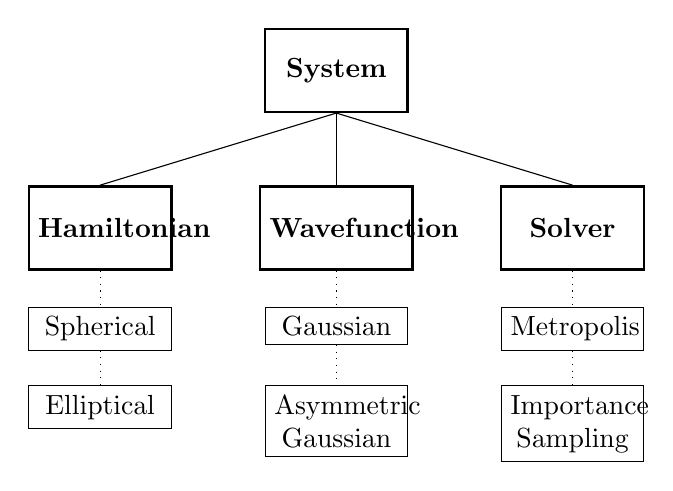
\begin{tikzpicture}
        
        \node (system) [draw, line width=0.3mm, text width=0.13\textwidth, minimum height=30pt, text centered] at (0,2) {\bfseries System};
        
        \node (wavefunction) [draw, line width=0.3mm, text width=0.14\textwidth, minimum height=30pt, text centered] at (0,0) {\bfseries Wavefunction};
        \node (gauss) [draw, anchor=north, text width=0.13\textwidth, text centered] at (0, -1) {Gaussian};
        \node (asymmgauss) [draw, anchor=north, text width=0.13\textwidth, text centered] at (0, -2) {Asymmetric \\ Gaussian};
        
        \node (solver) [draw, line width=0.3mm, text width=0.13\textwidth, minimum height=30pt, text centered] at (3,0) {\bfseries Solver};
        \node (metropolis) [draw, anchor=north, text width=0.13\textwidth, text centered] at (3, -1) {Metropolis};
        \node (importance) [draw, anchor=north, text width=0.13\textwidth, text centered] at (3, -2) {Importance \\ Sampling};
        
        \node (hamiltonian) [draw, line width=0.3mm, text width=0.13\textwidth, minimum height=30pt, text centered] at (-3,0) {\bfseries Hamiltonian};
        \node (spherical) [draw, anchor=north, text width=0.13\textwidth, text centered] at (-3, -1) {Spherical};
        \node (elliptical) [draw, anchor=north, text width=0.13\textwidth, text centered] at (-3, -2) {Elliptical};
        
        \draw (system.south) -- (wavefunction.north);
        \draw (system.south) -- (hamiltonian.north);
        \draw (system.south) -- (solver.north);
        
        \draw [dotted] (hamiltonian.south) -- (spherical.north);
        \draw [dotted] (spherical.south) -- (elliptical.north);
        \draw [dotted] (wavefunction.south) -- (gauss.north);
        \draw [dotted] (gauss.south) -- (asymmgauss.north);
        \draw [dotted] (solver.south) -- (metropolis.north);
        \draw [dotted] (metropolis.south) -- (importance.north);
    \end{tikzpicture}
    \caption{Classes diagram and hierarchy. Elliptical and spherical are Hamiltonian's subclasses, Gaussian and AsymmetricGaussian are Wavefunction's sublclasses, Metropolis and ImportanceSampling are Solver's sublasses.}
    \label{diag:classes_diagram}
\end{figure}
We chose C\texttt{++} as the main programming language to implement the aforementioned methods for this project. This allowed us to keep a good compromise between computational speed and abstraction. The algorithm has been fully object oriented making the code modular, in the sense one can in principle reuse the code for other purposes by only replacing some pieces and keeping the general structure. All the implemented classes can be classified into three categories:
\begin{itemize}
    \item \emph{System}: contains information on the system as a whole like the collection of particle and provides a reference point for communication between the other classes;
    \item \emph{Solvers} which provides different tools to evaluate the ground state of the chosen hamiltonian with the chosen wavefunction on different complexity levels, depending on the needs;
    \item \emph{Wavefunctions};
    \item \emph{Hamiltonians}.
\end{itemize}
The code has been documented via Doxygen and the documentation, together with the code itself, can be found at the GitHub link provided at the end of the report, hence hereby we discuss only some of the peculiar points of the implementation.
\subsection*{Wavefunction evaluation in the non-interacting case}
In the non-interacting case we exploited the relatively simple form of the local energy and the wavefunction to evaluate the Monte Carlo cycles in a more efficient way. In particular, at each cycle, we generated a proposal move for one particle only and evaluated the new wavefunction and the new local energy just by adjusting the values taken in the previous cycle since the dependence of each particle enters in the formulae only trough multiplicative factors or summation terms. To be more precise, if the wavefunction at the step $k$ of the algorithm is
$$\psi^{k} \equiv \psi(\bm{r}(t_k)) = \prod_{i=1}^{N} g(\alpha, \bm{r}_i(t_k)) \equiv \prod_{i=1}^N g_i^{(k)}$$
then, if at the step $k+1$ we modify the position of the particle $n$, the wavefunction becomes
$$\psi^{k+1} \ = \ g_n^{(k+1)} \, \prod_{\substack{i=1\\ i \neq n}} g_i^{k}$$
The relation for the local energy follows in a similar way.
\subsection*{Relative position in the interacting case}
The interacting case leads to way more complicated expressions and a clever way to evaluate the necessary quantities as done with the non-interacting case is not so immediate. However we noticed the repetitive demand for the same quantities, like the relative positions and relative distances between particles, in different expression, hence we stored those values in proper matrices avoiding repetitive re-evaluations of those high time-demanding operations. The $ij$-th element of the distance matrix $D_{ij}$ is the distance between the particle $i$ and particle $j$: here one can note that this matrix is symmetrical, hence only one half of the off-diagonal values must be computed. In a similar way the $ij$-th element of the relative position matrix $R_{ij} = \bm{r}_i - \bm{r}_j$ is the relative position, in cartesian coordinates, of the particles $i$ with respecto to the particle $j$: this matrix is antisymmetrical, hence, also in this case, only half of the off-diagonal element can be computed. The matrices are built and initialised at the beginning of the program, and after one particle is moved, only the corresponding rows and columns in the matrices are updated.
\subsubsection*{Code parallelization}
Various part of the code have been parallelized via OpenMP. \\
\dots Spiegare cosa e quali \dots 